\documentclass[1p]{elsarticle_modified}
%\bibliographystyle{elsarticle-num}

%\usepackage[colorlinks]{hyperref}
%\usepackage{abbrmath_seonhwa} %\Abb, \Ascr, \Acal ,\Abf, \Afrak
\usepackage{amsfonts}
\usepackage{amssymb}
\usepackage{amsmath}
\usepackage{amsthm}
\usepackage{scalefnt}
\usepackage{amsbsy}
\usepackage{kotex}
\usepackage{caption}
\usepackage{subfig}
\usepackage{color}
\usepackage{graphicx}
\usepackage{xcolor} %% white, black, red, green, blue, cyan, magenta, yellow
\usepackage{float}
\usepackage{setspace}
\usepackage{hyperref}

\usepackage{tikz}
\usetikzlibrary{arrows}

\usepackage{multirow}
\usepackage{array} % fixed length table
\usepackage{hhline}

%%%%%%%%%%%%%%%%%%%%%
\makeatletter
\renewcommand*\env@matrix[1][\arraystretch]{%
	\edef\arraystretch{#1}%
	\hskip -\arraycolsep
	\let\@ifnextchar\new@ifnextchar
	\array{*\c@MaxMatrixCols c}}
\makeatother %https://tex.stackexchange.com/questions/14071/how-can-i-increase-the-line-spacing-in-a-matrix
%%%%%%%%%%%%%%%

\usepackage[normalem]{ulem}

\newcommand{\msout}[1]{\ifmmode\text{\sout{\ensuremath{#1}}}\else\sout{#1}\fi}
%SOURCE: \msout is \stkout macro in https://tex.stackexchange.com/questions/20609/strikeout-in-math-mode

\newcommand{\cancel}[1]{
	\ifmmode
	{\color{red}\msout{#1}}
	\else
	{\color{red}\sout{#1}}
	\fi
}

\newcommand{\add}[1]{
	{\color{blue}\uwave{#1}}
}

\newcommand{\replace}[2]{
	\ifmmode
	{\color{red}\msout{#1}}{\color{blue}\uwave{#2}}
	\else
	{\color{red}\sout{#1}}{\color{blue}\uwave{#2}}
	\fi
}

\newcommand{\Sol}{\mathcal{S}} %segment
\newcommand{\D}{D} %diagram
\newcommand{\A}{\mathcal{A}} %arc


%%%%%%%%%%%%%%%%%%%%%%%%%%%%%5 test

\def\sl{\operatorname{\textup{SL}}(2,\Cbb)}
\def\psl{\operatorname{\textup{PSL}}(2,\Cbb)}
\def\quan{\mkern 1mu \triangleright \mkern 1mu}

\theoremstyle{definition}
\newtheorem{thm}{Theorem}[section]
\newtheorem{prop}[thm]{Proposition}
\newtheorem{lem}[thm]{Lemma}
\newtheorem{ques}[thm]{Question}
\newtheorem{cor}[thm]{Corollary}
\newtheorem{defn}[thm]{Definition}
\newtheorem{exam}[thm]{Example}
\newtheorem{rmk}[thm]{Remark}
\newtheorem{alg}[thm]{Algorithm}

\newcommand{\I}{\sqrt{-1}}
\begin{document}

%\begin{frontmatter}
%
%\title{Boundary parabolic representations of knots up to 8 crossings}
%
%%% Group authors per affiliation:
%\author{Yunhi Cho} 
%\address{Department of Mathematics, University of Seoul, Seoul, Korea}
%\ead{yhcho@uos.ac.kr}
%
%
%\author{Seonhwa Kim} %\fnref{s_kim}}
%\address{Center for Geometry and Physics, Institute for Basic Science, Pohang, 37673, Korea}
%\ead{ryeona17@ibs.re.kr}
%
%\author{Hyuk Kim}
%\address{Department of Mathematical Sciences, Seoul National University, Seoul 08826, Korea}
%\ead{hyukkim@snu.ac.kr}
%
%\author{Seokbeom Yoon}
%\address{Department of Mathematical Sciences, Seoul National University, Seoul, 08826,  Korea}
%\ead{sbyoon15@snu.ac.kr}
%
%\begin{abstract}
%We find all boundary parabolic representation of knots up to 8 crossings.
%
%\end{abstract}
%\begin{keyword}
%    \MSC[2010] 57M25 
%\end{keyword}
%
%\end{frontmatter}

%\linenumbers
%\tableofcontents
%
\newcommand\colored[1]{\textcolor{white}{\rule[-0.35ex]{0.8em}{1.4ex}}\kern-0.8em\color{red} #1}%
%\newcommand\colored[1]{\textcolor{white}{ #1}\kern-2.17ex	\textcolor{white}{ #1}\kern-1.81ex	\textcolor{white}{ #1}\kern-2.15ex\color{red}#1	}

{\Large $\underline{10_{165}~(K10n_{37})}$}

\setlength{\tabcolsep}{10pt}
\renewcommand{\arraystretch}{1.6}
\vspace{1cm}\begin{tabular}{m{100pt}>{\centering\arraybackslash}m{274pt}}
\multirow{5}{120pt}{
	\centering
	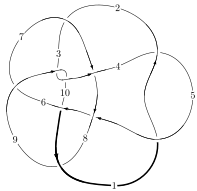
\includegraphics[width=112pt]{../../../GIT/diagram.site/Diagrams/png/249_10_165.png}\\
\ \ \ A knot diagram\footnotemark}&
\allowdisplaybreaks
\textbf{Linearized knot diagam} \\
\cline{2-2}
 &
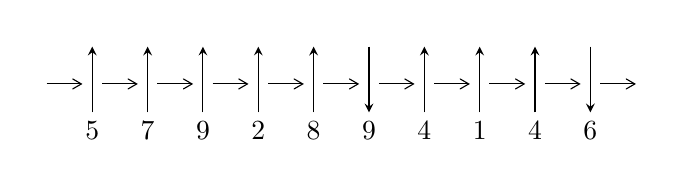
\begin{tikzpicture}[x=20pt, y=17pt]
	% nodes
	\node (C0) at (0, 0) {};
	\node (C1) at (1, 0) {};
	\node (C1U) at (1, +1) {};
	\node (C1D) at (1, -1) {5};

	\node (C2) at (2, 0) {};
	\node (C2U) at (2, +1) {};
	\node (C2D) at (2, -1) {7};

	\node (C3) at (3, 0) {};
	\node (C3U) at (3, +1) {};
	\node (C3D) at (3, -1) {9};

	\node (C4) at (4, 0) {};
	\node (C4U) at (4, +1) {};
	\node (C4D) at (4, -1) {2};

	\node (C5) at (5, 0) {};
	\node (C5U) at (5, +1) {};
	\node (C5D) at (5, -1) {8};

	\node (C6) at (6, 0) {};
	\node (C6U) at (6, +1) {};
	\node (C6D) at (6, -1) {9};

	\node (C7) at (7, 0) {};
	\node (C7U) at (7, +1) {};
	\node (C7D) at (7, -1) {4};

	\node (C8) at (8, 0) {};
	\node (C8U) at (8, +1) {};
	\node (C8D) at (8, -1) {1};

	\node (C9) at (9, 0) {};
	\node (C9U) at (9, +1) {};
	\node (C9D) at (9, -1) {4};

	\node (C10) at (10, 0) {};
	\node (C10U) at (10, +1) {};
	\node (C10D) at (10, -1) {6};
	\node (C11) at (11, 0) {};

	% arrows
	\draw[->,>={angle 60}]
	(C0) edge (C1) (C1) edge (C2) (C2) edge (C3) (C3) edge (C4) (C4) edge (C5) (C5) edge (C6) (C6) edge (C7) (C7) edge (C8) (C8) edge (C9) (C9) edge (C10) (C10) edge (C11) ;	\draw[->,>=stealth]
	(C1D) edge (C1U) (C2D) edge (C2U) (C3D) edge (C3U) (C4D) edge (C4U) (C5D) edge (C5U) (C6U) edge (C6D) (C7D) edge (C7U) (C8D) edge (C8U) (C9D) edge (C9U) (C10U) edge (C10D) ;
	\end{tikzpicture} \\
\hhline{~~} \\& 
\textbf{Solving Sequence} \\ \cline{2-2} 
 &
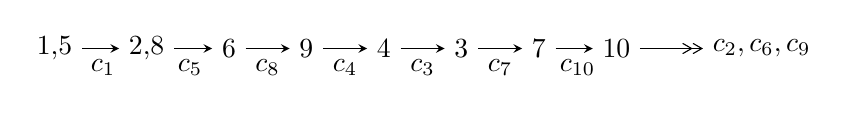
\begin{tikzpicture}[x=28pt, y=7pt]
	% node
	\node (A0) at (-1/8, 0) {1,5};
	\node (A1) at (17/16, 0) {2,8};
	\node (A2) at (17/8, 0) {6};
	\node (A3) at (25/8, 0) {9};
	\node (A4) at (33/8, 0) {4};
	\node (A5) at (41/8, 0) {3};
	\node (A6) at (49/8, 0) {7};
	\node (A7) at (57/8, 0) {10};
	\node (C1) at (1/2, -1) {$c_{1}$};
	\node (C2) at (13/8, -1) {$c_{5}$};
	\node (C3) at (21/8, -1) {$c_{8}$};
	\node (C4) at (29/8, -1) {$c_{4}$};
	\node (C5) at (37/8, -1) {$c_{3}$};
	\node (C6) at (45/8, -1) {$c_{7}$};
	\node (C7) at (53/8, -1) {$c_{10}$};
	\node (A8) at (9, 0) {$c_{2},c_{6},c_{9}$};

	% edge
	\draw[->,>=stealth]	
	(A0) edge (A1) (A1) edge (A2) (A2) edge (A3) (A3) edge (A4) (A4) edge (A5) (A5) edge (A6) (A6) edge (A7) ;
	\draw[->>,>={angle 60}]	
	(A7) edge (A8);
\end{tikzpicture} \\ 

\end{tabular} \\

\footnotetext{
The image of knot diagram is generated by the software ``\textbf{Draw programme}" developed by Andrew Bartholomew(\url{http://www.layer8.co.uk/maths/draw/index.htm\#Running-draw}), where we modified some parts for our purpose(\url{https://github.com/CATsTAILs/LinksPainter}).
}\phantom \\ \newline 
\centering \textbf{Ideals for irreducible components\footnotemark of $X_{\text{par}}$} 
 
\begin{align*}
I^u_{1}&=\langle 
u^{12}+5 u^{11}+16 u^{10}+34 u^9+53 u^8+61 u^7+48 u^6+20 u^5-9 u^4-24 u^3-20 u^2+b-11 u-3,\\
\phantom{I^u_{1}}&\phantom{= \langle  }-3 u^{12}-13 u^{11}-41 u^{10}-85 u^9-136 u^8-167 u^7-148 u^6-90 u^5-5 u^4+54 u^3+63 u^2+2 a+50 u+14,\\
\phantom{I^u_{1}}&\phantom{= \langle  }u^{13}+5 u^{12}+17 u^{11}+39 u^{10}+68 u^9+91 u^8+90 u^7+62 u^6+15 u^5-24 u^4-37 u^3-30 u^2-12 u-2\rangle \\
I^u_{2}&=\langle 
- u^3- u^2+b- u-1,\;u^5+2 u^4+4 u^3+3 u^2+2 a+3 u+2,\;u^6+2 u^5+4 u^4+5 u^3+5 u^2+4 u+2\rangle \\
I^u_{3}&=\langle 
- u^5+u^4-2 u^3+a u+u^2+b- u+1,\\
\phantom{I^u_{3}}&\phantom{= \langle  }u^5 a-2 u^4 a-2 u^5+4 u^3 a+3 u^4-4 u^2 a-7 u^3+a^2+3 a u+7 u^2-2 a-6 u+4,\\
\phantom{I^u_{3}}&\phantom{= \langle  }u^6- u^5+3 u^4-2 u^3+2 u^2- u-1\rangle \\
\\
\end{align*}
\raggedright * 3 irreducible components of $\dim_{\mathbb{C}}=0$, with total 31 representations.\\
\footnotetext{All coefficients of polynomials are rational numbers. But the coefficients are sometimes approximated in decimal forms when there is not enough margin.}
\newpage
\renewcommand{\arraystretch}{1}
\centering \section*{I. $I^u_{1}= \langle u^{12}+5 u^{11}+\cdots+b-3,\;-3 u^{12}-13 u^{11}+\cdots+2 a+14,\;u^{13}+5 u^{12}+\cdots-12 u-2 \rangle$}
\flushleft \textbf{(i) Arc colorings}\\
\begin{tabular}{m{7pt} m{180pt} m{7pt} m{180pt} }
\flushright $a_{1}=$&$\begin{pmatrix}1\\0\end{pmatrix}$ \\
\flushright $a_{5}=$&$\begin{pmatrix}0\\u\end{pmatrix}$ \\
\flushright $a_{2}=$&$\begin{pmatrix}1\\- u^2\end{pmatrix}$ \\
\flushright $a_{8}=$&$\begin{pmatrix}\frac{3}{2} u^{12}+\frac{13}{2} u^{11}+\cdots-25 u-7\\- u^{12}-5 u^{11}+\cdots+11 u+3\end{pmatrix}$ \\
\flushright $a_{6}=$&$\begin{pmatrix}\frac{3}{2} u^{12}+\frac{13}{2} u^{11}+\cdots-20 u-4\\- u^{12}-5 u^{11}+\cdots+15 u+3\end{pmatrix}$ \\
\flushright $a_{9}=$&$\begin{pmatrix}\frac{1}{2} u^{12}+\frac{3}{2} u^{11}+\cdots-14 u-4\\- u^{12}-5 u^{11}+\cdots+11 u+3\end{pmatrix}$ \\
\flushright $a_{4}=$&$\begin{pmatrix}- u\\u^3+u\end{pmatrix}$ \\
\flushright $a_{3}=$&$\begin{pmatrix}\frac{1}{2} u^{12}+\frac{5}{2} u^{11}+\cdots-4 u-1\\u^{12}+4 u^{11}+\cdots-5 u-1\end{pmatrix}$ \\
\flushright $a_{7}=$&$\begin{pmatrix}\frac{1}{2} u^{12}+\frac{5}{2} u^{11}+\cdots-26 u-7\\- u^{12}-4 u^{11}+\cdots+2 u+1\end{pmatrix}$ \\
\flushright $a_{10}=$&$\begin{pmatrix}\frac{1}{2} u^{12}+\frac{3}{2} u^{11}+\cdots-13 u-4\\- u^{12}-5 u^{11}+\cdots+10 u+3\end{pmatrix}$\\&\end{tabular}
\flushleft \textbf{(ii) Obstruction class $= -1$}\\~\\
\flushleft \textbf{(iii) Cusp Shapes $= 5 u^{12}+24 u^{11}+78 u^{10}+170 u^9+277 u^8+342 u^7+296 u^6+161 u^5-15 u^4-125 u^3-126 u^2-82 u-16$}\\~\\
\newpage\renewcommand{\arraystretch}{1}
\flushleft \textbf{(iv) u-Polynomials at the component}\newline \\
\begin{tabular}{m{50pt}|m{274pt}}
Crossings & \hspace{64pt}u-Polynomials at each crossing \\
\hline $$\begin{aligned}c_{1},c_{4}\end{aligned}$$&$\begin{aligned}
&u^{13}+5 u^{12}+\cdots-12 u-2
\end{aligned}$\\
\hline $$\begin{aligned}c_{2},c_{3},c_{9}\end{aligned}$$&$\begin{aligned}
&u^{13}+10 u^{11}+\cdots+2 u-1
\end{aligned}$\\
\hline $$\begin{aligned}c_{5},c_{8}\end{aligned}$$&$\begin{aligned}
&u^{13}+u^{12}+\cdots+5 u-1
\end{aligned}$\\
\hline $$\begin{aligned}c_{6}\end{aligned}$$&$\begin{aligned}
&u^{13}-8 u^{12}+\cdots+18 u-10
\end{aligned}$\\
\hline $$\begin{aligned}c_{7}\end{aligned}$$&$\begin{aligned}
&u^{13}- u^{12}+\cdots+20 u-7
\end{aligned}$\\
\hline $$\begin{aligned}c_{10}\end{aligned}$$&$\begin{aligned}
&u^{13}+12 u^{12}+\cdots-288 u-64
\end{aligned}$\\
\hline
\end{tabular}\\~\\
\newpage\renewcommand{\arraystretch}{1}
\flushleft \textbf{(v) Riley Polynomials at the component}\newline \\
\begin{tabular}{m{50pt}|m{274pt}}
Crossings & \hspace{64pt}Riley Polynomials at each crossing \\
\hline $$\begin{aligned}c_{1},c_{4}\end{aligned}$$&$\begin{aligned}
&y^{13}+9 y^{12}+\cdots+24 y-4
\end{aligned}$\\
\hline $$\begin{aligned}c_{2},c_{3},c_{9}\end{aligned}$$&$\begin{aligned}
&y^{13}+20 y^{12}+\cdots-10 y-1
\end{aligned}$\\
\hline $$\begin{aligned}c_{5},c_{8}\end{aligned}$$&$\begin{aligned}
&y^{13}+7 y^{12}+\cdots+23 y-1
\end{aligned}$\\
\hline $$\begin{aligned}c_{6}\end{aligned}$$&$\begin{aligned}
&y^{13}-16 y^{12}+\cdots+1284 y-100
\end{aligned}$\\
\hline $$\begin{aligned}c_{7}\end{aligned}$$&$\begin{aligned}
&y^{13}+13 y^{12}+\cdots+64 y-49
\end{aligned}$\\
\hline $$\begin{aligned}c_{10}\end{aligned}$$&$\begin{aligned}
&y^{13}-2 y^{12}+\cdots+1024 y-4096
\end{aligned}$\\
\hline
\end{tabular}\\~\\
\newpage\flushleft \textbf{(vi) Complex Volumes and Cusp Shapes}
$$\begin{array}{c|c|c}  
\text{Solutions to }I^u_{1}& \I (\text{vol} + \sqrt{-1}CS) & \text{Cusp shape}\\
 \hline 
\begin{aligned}
u &= -1.152860 + 0.170520 I \\
a &= \phantom{-}0.717142 - 0.770562 I \\
b &= -0.695367 + 1.010640 I\end{aligned}
 & -6.75019 - 5.87953 I & \phantom{-}3.71309 + 4.79533 I \\ \hline\begin{aligned}
u &= -1.152860 - 0.170520 I \\
a &= \phantom{-}0.717142 + 0.770562 I \\
b &= -0.695367 - 1.010640 I\end{aligned}
 & -6.75019 + 5.87953 I & \phantom{-}3.71309 - 4.79533 I \\ \hline\begin{aligned}
u &= -0.034812 + 1.171400 I \\
a &= \phantom{-}0.739139 + 0.284263 I \\
b &= -0.358718 + 0.855935 I\end{aligned}
 & -3.39029 + 0.96735 I & \phantom{-}2.31477 - 3.00161 I \\ \hline\begin{aligned}
u &= -0.034812 - 1.171400 I \\
a &= \phantom{-}0.739139 - 0.284263 I \\
b &= -0.358718 - 0.855935 I\end{aligned}
 & -3.39029 - 0.96735 I & \phantom{-}2.31477 + 3.00161 I \\ \hline\begin{aligned}
u &= -0.175701 + 1.175030 I \\
a &= -1.067580 - 0.632688 I \\
b &= \phantom{-}0.93100 - 1.14328 I\end{aligned}
 & -2.32319 - 3.89550 I & \phantom{-}2.16216 + 1.95849 I \\ \hline\begin{aligned}
u &= -0.175701 - 1.175030 I \\
a &= -1.067580 + 0.632688 I \\
b &= \phantom{-}0.93100 + 1.14328 I\end{aligned}
 & -2.32319 + 3.89550 I & \phantom{-}2.16216 - 1.95849 I \\ \hline\begin{aligned}
u &= \phantom{-}0.773330\phantom{ +0.000000I} \\
a &= \phantom{-}0.244870\phantom{ +0.000000I} \\
b &= \phantom{-}0.189365\phantom{ +0.000000I}\end{aligned}
 & \phantom{-}1.09959\phantom{ +0.000000I} & \phantom{-}6.33360\phantom{ +0.000000I} \\ \hline\begin{aligned}
u &= -0.48596 + 1.43258 I \\
a &= \phantom{-}1.058960 + 0.295073 I \\
b &= -0.93732 + 1.37365 I\end{aligned}
 & -11.8216 - 11.6031 I & \phantom{-}1.77641 + 5.73851 I \\ \hline\begin{aligned}
u &= -0.48596 - 1.43258 I \\
a &= \phantom{-}1.058960 - 0.295073 I \\
b &= -0.93732 - 1.37365 I\end{aligned}
 & -11.8216 + 11.6031 I & \phantom{-}1.77641 - 5.73851 I \\ \hline\begin{aligned}
u &= -0.363253 + 0.187651 I \\
a &= -0.56911 - 2.04054 I \\
b &= \phantom{-}0.589641 + 0.634441 I\end{aligned}
 & \phantom{-}0.57483 + 1.68891 I & \phantom{-}3.43240 - 5.42565 I\\
 \hline 
 \end{array}$$\newpage$$\begin{array}{c|c|c}  
\text{Solutions to }I^u_{1}& \I (\text{vol} + \sqrt{-1}CS) & \text{Cusp shape}\\
 \hline 
\begin{aligned}
u &= -0.363253 - 0.187651 I \\
a &= -0.56911 + 2.04054 I \\
b &= \phantom{-}0.589641 - 0.634441 I\end{aligned}
 & \phantom{-}0.57483 - 1.68891 I & \phantom{-}3.43240 + 5.42565 I \\ \hline\begin{aligned}
u &= -0.67408 + 1.45370 I \\
a &= -0.500985 + 0.317553 I \\
b &= -0.123919 - 0.942337 I\end{aligned}
 & -10.56050 - 0.87235 I & -1.56565 + 0.23907 I \\ \hline\begin{aligned}
u &= -0.67408 - 1.45370 I \\
a &= -0.500985 - 0.317553 I \\
b &= -0.123919 + 0.942337 I\end{aligned}
 & -10.56050 + 0.87235 I & -1.56565 - 0.23907 I\\
 \hline 
 \end{array}$$\newpage\newpage\renewcommand{\arraystretch}{1}
\centering \section*{II. $I^u_{2}= \langle - u^3- u^2+b- u-1,\;u^5+2 u^4+4 u^3+3 u^2+2 a+3 u+2,\;u^6+2 u^5+4 u^4+5 u^3+5 u^2+4 u+2 \rangle$}
\flushleft \textbf{(i) Arc colorings}\\
\begin{tabular}{m{7pt} m{180pt} m{7pt} m{180pt} }
\flushright $a_{1}=$&$\begin{pmatrix}1\\0\end{pmatrix}$ \\
\flushright $a_{5}=$&$\begin{pmatrix}0\\u\end{pmatrix}$ \\
\flushright $a_{2}=$&$\begin{pmatrix}1\\- u^2\end{pmatrix}$ \\
\flushright $a_{8}=$&$\begin{pmatrix}-\frac{1}{2} u^5- u^4-2 u^3-\frac{3}{2} u^2-\frac{3}{2} u-1\\u^3+u^2+u+1\end{pmatrix}$ \\
\flushright $a_{6}=$&$\begin{pmatrix}\frac{1}{2} u^5+u^4+u^3+\frac{3}{2} u^2+\frac{1}{2} u\\- u^4- u^3-2 u^2- u-1\end{pmatrix}$ \\
\flushright $a_{9}=$&$\begin{pmatrix}-\frac{1}{2} u^5- u^4- u^3-\frac{1}{2} u^2-\frac{1}{2} u\\u^3+u^2+u+1\end{pmatrix}$ \\
\flushright $a_{4}=$&$\begin{pmatrix}- u\\u^3+u\end{pmatrix}$ \\
\flushright $a_{3}=$&$\begin{pmatrix}\frac{1}{2} u^5+2 u^4+3 u^3+\frac{7}{2} u^2+\frac{3}{2} u+1\\u^5+2 u^4+4 u^3+3 u^2+3 u+1\end{pmatrix}$ \\
\flushright $a_{7}=$&$\begin{pmatrix}-\frac{1}{2} u^5+\frac{3}{2} u^2+\frac{3}{2} u+1\\u^3+u^2+2 u+1\end{pmatrix}$ \\
\flushright $a_{10}=$&$\begin{pmatrix}-\frac{1}{2} u^5- u^4-2 u^3-\frac{3}{2} u^2-\frac{3}{2} u\\u^5+u^4+3 u^3+2 u^2+2 u+1\end{pmatrix}$\\&\end{tabular}
\flushleft \textbf{(ii) Obstruction class $= 1$}\\~\\
\flushleft \textbf{(iii) Cusp Shapes $= 5 u^4+4 u^3+9 u^2+6 u+10$}\\~\\
\newpage\renewcommand{\arraystretch}{1}
\flushleft \textbf{(iv) u-Polynomials at the component}\newline \\
\begin{tabular}{m{50pt}|m{274pt}}
Crossings & \hspace{64pt}u-Polynomials at each crossing \\
\hline $$\begin{aligned}c_{1}\end{aligned}$$&$\begin{aligned}
&u^6+2 u^5+4 u^4+5 u^3+5 u^2+4 u+2
\end{aligned}$\\
\hline $$\begin{aligned}c_{2},c_{3},c_{9}\end{aligned}$$&$\begin{aligned}
&u^6+2 u^4-2 u^2+1
\end{aligned}$\\
\hline $$\begin{aligned}c_{4}\end{aligned}$$&$\begin{aligned}
&u^6-2 u^5+4 u^4-5 u^3+5 u^2-4 u+2
\end{aligned}$\\
\hline $$\begin{aligned}c_{5},c_{8},c_{10}\end{aligned}$$&$\begin{aligned}
&u^6+u^5-2 u^3+u+1
\end{aligned}$\\
\hline $$\begin{aligned}c_{6}\end{aligned}$$&$\begin{aligned}
&u^6-5 u^5+10 u^4-12 u^3+11 u^2-6 u+2
\end{aligned}$\\
\hline $$\begin{aligned}c_{7}\end{aligned}$$&$\begin{aligned}
&u^6+u^5+3 u^4- u^3+u^2-2 u+1
\end{aligned}$\\
\hline
\end{tabular}\\~\\
\newpage\renewcommand{\arraystretch}{1}
\flushleft \textbf{(v) Riley Polynomials at the component}\newline \\
\begin{tabular}{m{50pt}|m{274pt}}
Crossings & \hspace{64pt}Riley Polynomials at each crossing \\
\hline $$\begin{aligned}c_{1},c_{4}\end{aligned}$$&$\begin{aligned}
&y^6+4 y^5+6 y^4+3 y^3+y^2+4 y+4
\end{aligned}$\\
\hline $$\begin{aligned}c_{2},c_{3},c_{9}\end{aligned}$$&$\begin{aligned}
&(y^3+2 y^2-2 y+1)^2
\end{aligned}$\\
\hline $$\begin{aligned}c_{5},c_{8},c_{10}\end{aligned}$$&$\begin{aligned}
&y^6- y^5+4 y^4-4 y^3+4 y^2- y+1
\end{aligned}$\\
\hline $$\begin{aligned}c_{6}\end{aligned}$$&$\begin{aligned}
&y^6-5 y^5+2 y^4+20 y^3+17 y^2+8 y+4
\end{aligned}$\\
\hline $$\begin{aligned}c_{7}\end{aligned}$$&$\begin{aligned}
&y^6+5 y^5+13 y^4+11 y^3+3 y^2-2 y+1
\end{aligned}$\\
\hline
\end{tabular}\\~\\
\newpage\flushleft \textbf{(vi) Complex Volumes and Cusp Shapes}
$$\begin{array}{c|c|c}  
\text{Solutions to }I^u_{2}& \I (\text{vol} + \sqrt{-1}CS) & \text{Cusp shape}\\
 \hline 
\begin{aligned}
u &= -0.862023 + 0.412869 I \\
a &= -0.233003 - 0.750879 I \\
b &= \phantom{-}0.510869 + 0.551075 I\end{aligned}
 & \phantom{-}1.44750 + 0.78507 I & \phantom{-}8.28869 - 4.60495 I \\ \hline\begin{aligned}
u &= -0.862023 - 0.412869 I \\
a &= -0.233003 + 0.750879 I \\
b &= \phantom{-}0.510869 - 0.551075 I\end{aligned}
 & \phantom{-}1.44750 - 0.78507 I & \phantom{-}8.28869 + 4.60495 I \\ \hline\begin{aligned}
u &= \phantom{-}0.238984 + 1.138460 I \\
a &= \phantom{-}0.176605 + 0.841305 I \\
b &= -0.915589 + 0.402116 I\end{aligned}
 & -8.28528 + 1.18132 I & \phantom{-}2.81561 - 0.13577 I \\ \hline\begin{aligned}
u &= \phantom{-}0.238984 - 1.138460 I \\
a &= \phantom{-}0.176605 - 0.841305 I \\
b &= -0.915589 - 0.402116 I\end{aligned}
 & -8.28528 - 1.18132 I & \phantom{-}2.81561 + 0.13577 I \\ \hline\begin{aligned}
u &= -0.376961 + 1.214800 I \\
a &= -0.943602 - 0.451942 I \\
b &= \phantom{-}0.904720 - 0.975923 I\end{aligned}
 & -1.38689 - 5.20040 I & \phantom{-}6.89570 + 6.16090 I \\ \hline\begin{aligned}
u &= -0.376961 - 1.214800 I \\
a &= -0.943602 + 0.451942 I \\
b &= \phantom{-}0.904720 + 0.975923 I\end{aligned}
 & -1.38689 + 5.20040 I & \phantom{-}6.89570 - 6.16090 I\\
 \hline 
 \end{array}$$\newpage\newpage\renewcommand{\arraystretch}{1}
\centering \section*{III. $I^u_{3}= \langle - u^5+u^4-2 u^3+a u+u^2+b- u+1,\;u^5 a-2 u^5+\cdots-2 a+4,\;u^6- u^5+3 u^4-2 u^3+2 u^2- u-1 \rangle$}
\flushleft \textbf{(i) Arc colorings}\\
\begin{tabular}{m{7pt} m{180pt} m{7pt} m{180pt} }
\flushright $a_{1}=$&$\begin{pmatrix}1\\0\end{pmatrix}$ \\
\flushright $a_{5}=$&$\begin{pmatrix}0\\u\end{pmatrix}$ \\
\flushright $a_{2}=$&$\begin{pmatrix}1\\- u^2\end{pmatrix}$ \\
\flushright $a_{8}=$&$\begin{pmatrix}a\\u^5- u^4+2 u^3- a u- u^2+u-1\end{pmatrix}$ \\
\flushright $a_{6}=$&$\begin{pmatrix}u^5 a- u^4 a- u^5+2 u^3 a+u^4- u^2 a-3 u^3+a u+2 u^2- a-2 u+2\\1\end{pmatrix}$ \\
\flushright $a_{9}=$&$\begin{pmatrix}u^5- u^4+2 u^3- a u- u^2+a+u-1\\u^5- u^4+2 u^3- a u- u^2+u-1\end{pmatrix}$ \\
\flushright $a_{4}=$&$\begin{pmatrix}- u\\u^3+u\end{pmatrix}$ \\
\flushright $a_{3}=$&$\begin{pmatrix}u^5-3 u^4+6 u^3- a u-7 u^2+a+5 u-3\\u^3 a-2 u^4- u^2 a+3 u^3+a u-3 u^2+2 u+1\end{pmatrix}$ \\
\flushright $a_{7}=$&$\begin{pmatrix}- u^4 a+u^5+u^3 a- u^4- u^2 a+u^3+a- u\\- u^4 a+2 u^5+u^3 a-2 u^4- u^2 a+4 u^3-2 u^2+a+u-1\end{pmatrix}$ \\
\flushright $a_{10}=$&$\begin{pmatrix}- u^5 a+u^4 a+u^5-2 u^3 a- u^4+u^2 a+3 u^3- a u-2 u^2+a+2 u-1\\-1\end{pmatrix}$\\&\end{tabular}
\flushleft \textbf{(ii) Obstruction class $= -1$}\\~\\
\flushleft \textbf{(iii) Cusp Shapes $= 4 u^4-4 u^3+8 u^2-4 u+2$}\\~\\
\newpage\renewcommand{\arraystretch}{1}
\flushleft \textbf{(iv) u-Polynomials at the component}\newline \\
\begin{tabular}{m{50pt}|m{274pt}}
Crossings & \hspace{64pt}u-Polynomials at each crossing \\
\hline $$\begin{aligned}c_{1},c_{4}\end{aligned}$$&$\begin{aligned}
&(u^6- u^5+3 u^4-2 u^3+2 u^2- u-1)^2
\end{aligned}$\\
\hline $$\begin{aligned}c_{2},c_{3},c_{9}\end{aligned}$$&$\begin{aligned}
&u^{12}+u^{11}+\cdots+2 u+13
\end{aligned}$\\
\hline $$\begin{aligned}c_{5},c_{8}\end{aligned}$$&$\begin{aligned}
&u^{12}+5 u^{11}+\cdots+6 u^2+1
\end{aligned}$\\
\hline $$\begin{aligned}c_{6}\end{aligned}$$&$\begin{aligned}
&(u^6+5 u^5+7 u^4-2 u^2+3 u-1)^2
\end{aligned}$\\
\hline $$\begin{aligned}c_{7}\end{aligned}$$&$\begin{aligned}
&u^{12}- u^{11}+\cdots-18 u+23
\end{aligned}$\\
\hline $$\begin{aligned}c_{10}\end{aligned}$$&$\begin{aligned}
&(u-1)^{12}
\end{aligned}$\\
\hline
\end{tabular}\\~\\
\newpage\renewcommand{\arraystretch}{1}
\flushleft \textbf{(v) Riley Polynomials at the component}\newline \\
\begin{tabular}{m{50pt}|m{274pt}}
Crossings & \hspace{64pt}Riley Polynomials at each crossing \\
\hline $$\begin{aligned}c_{1},c_{4}\end{aligned}$$&$\begin{aligned}
&(y^6+5 y^5+9 y^4+4 y^3-6 y^2-5 y+1)^2
\end{aligned}$\\
\hline $$\begin{aligned}c_{2},c_{3},c_{9}\end{aligned}$$&$\begin{aligned}
&y^{12}+15 y^{11}+\cdots+360 y+169
\end{aligned}$\\
\hline $$\begin{aligned}c_{5},c_{8}\end{aligned}$$&$\begin{aligned}
&y^{12}- y^{11}+\cdots+12 y+1
\end{aligned}$\\
\hline $$\begin{aligned}c_{6}\end{aligned}$$&$\begin{aligned}
&(y^6-11 y^5+45 y^4-60 y^3-10 y^2-5 y+1)^2
\end{aligned}$\\
\hline $$\begin{aligned}c_{7}\end{aligned}$$&$\begin{aligned}
&y^{12}+11 y^{11}+\cdots-416 y+529
\end{aligned}$\\
\hline $$\begin{aligned}c_{10}\end{aligned}$$&$\begin{aligned}
&(y-1)^{12}
\end{aligned}$\\
\hline
\end{tabular}\\~\\
\newpage\flushleft \textbf{(vi) Complex Volumes and Cusp Shapes}
$$\begin{array}{c|c|c}  
\text{Solutions to }I^u_{3}& \I (\text{vol} + \sqrt{-1}CS) & \text{Cusp shape}\\
 \hline 
\begin{aligned}
u &= \phantom{-}0.873214\phantom{ +0.000000I} \\
a &= \phantom{-}0.211090 + 0.348879 I \\
b &= \phantom{-}0.184327 - 0.304646 I\end{aligned}
 & \phantom{-}1.08035\phantom{ +0.000000I} & \phantom{-}4.26950\phantom{ +0.000000I} \\ \hline\begin{aligned}
u &= \phantom{-}0.873214\phantom{ +0.000000I} \\
a &= \phantom{-}0.211090 - 0.348879 I \\
b &= \phantom{-}0.184327 + 0.304646 I\end{aligned}
 & \phantom{-}1.08035\phantom{ +0.000000I} & \phantom{-}4.26950\phantom{ +0.000000I} \\ \hline\begin{aligned}
u &= -0.138835 + 1.234450 I \\
a &= \phantom{-}0.576096 + 0.033593 I \\
b &= -1.96628 - 1.27394 I\end{aligned}
 & -9.53998 - 1.97241 I & -3.42428 + 3.68478 I \\ \hline\begin{aligned}
u &= -0.138835 + 1.234450 I \\
a &= -0.84220 + 1.68756 I \\
b &= -0.121451 + 0.706495 I\end{aligned}
 & -9.53998 - 1.97241 I & -3.42428 + 3.68478 I \\ \hline\begin{aligned}
u &= -0.138835 - 1.234450 I \\
a &= \phantom{-}0.576096 - 0.033593 I \\
b &= -1.96628 + 1.27394 I\end{aligned}
 & -9.53998 + 1.97241 I & -3.42428 - 3.68478 I \\ \hline\begin{aligned}
u &= -0.138835 - 1.234450 I \\
a &= -0.84220 - 1.68756 I \\
b &= -0.121451 - 0.706495 I\end{aligned}
 & -9.53998 + 1.97241 I & -3.42428 - 3.68478 I \\ \hline\begin{aligned}
u &= \phantom{-}0.408802 + 1.276380 I \\
a &= \phantom{-}1.089440 - 0.275882 I \\
b &= -0.511061 - 0.781659 I\end{aligned}
 & -2.88416 + 4.59213 I & \phantom{-}0.58114 - 3.20482 I \\ \hline\begin{aligned}
u &= \phantom{-}0.408802 + 1.276380 I \\
a &= -0.671738 + 0.185253 I \\
b &= \phantom{-}0.79749 + 1.27775 I\end{aligned}
 & -2.88416 + 4.59213 I & \phantom{-}0.58114 - 3.20482 I \\ \hline\begin{aligned}
u &= \phantom{-}0.408802 - 1.276380 I \\
a &= \phantom{-}1.089440 + 0.275882 I \\
b &= -0.511061 + 0.781659 I\end{aligned}
 & -2.88416 - 4.59213 I & \phantom{-}0.58114 + 3.20482 I \\ \hline\begin{aligned}
u &= \phantom{-}0.408802 - 1.276380 I \\
a &= -0.671738 - 0.185253 I \\
b &= \phantom{-}0.79749 - 1.27775 I\end{aligned}
 & -2.88416 - 4.59213 I & \phantom{-}0.58114 + 3.20482 I\\
 \hline 
 \end{array}$$\newpage$$\begin{array}{c|c|c}  
\text{Solutions to }I^u_{3}& \I (\text{vol} + \sqrt{-1}CS) & \text{Cusp shape}\\
 \hline 
\begin{aligned}
u &= -0.413150\phantom{ +0.000000I} \\
a &= \phantom{-}2.13731 + 1.92634 I \\
b &= -0.883031 + 0.795869 I\end{aligned}
 & -5.84089\phantom{ +0.000000I} & \phantom{-}5.41680\phantom{ +0.000000I} \\ \hline\begin{aligned}
u &= -0.413150\phantom{ +0.000000I} \\
a &= \phantom{-}2.13731 - 1.92634 I \\
b &= -0.883031 - 0.795869 I\end{aligned}
 & -5.84089\phantom{ +0.000000I} & \phantom{-}5.41680\phantom{ +0.000000I}\\
 \hline 
 \end{array}$$\newpage
\newpage\renewcommand{\arraystretch}{1}
\centering \section*{ IV. u-Polynomials}
\begin{tabular}{m{50pt}|m{274pt}}
Crossings & \hspace{64pt}u-Polynomials at each crossing \\
\hline $$\begin{aligned}c_{1}\end{aligned}$$&$\begin{aligned}
&(u^6- u^5+3 u^4-2 u^3+2 u^2- u-1)^2\\
&\cdot(u^6+2 u^5+\cdots+4 u+2)(u^{13}+5 u^{12}+\cdots-12 u-2)
\end{aligned}$\\
\hline $$\begin{aligned}c_{2},c_{3},c_{9}\end{aligned}$$&$\begin{aligned}
&(u^6+2 u^4-2 u^2+1)(u^{12}+u^{11}+\cdots+2 u+13)\\
&\cdot(u^{13}+10 u^{11}+\cdots+2 u-1)
\end{aligned}$\\
\hline $$\begin{aligned}c_{4}\end{aligned}$$&$\begin{aligned}
&(u^6-2 u^5+4 u^4-5 u^3+5 u^2-4 u+2)\\
&\cdot((u^6- u^5+3 u^4-2 u^3+2 u^2- u-1)^{2})(u^{13}+5 u^{12}+\cdots-12 u-2)
\end{aligned}$\\
\hline $$\begin{aligned}c_{5},c_{8}\end{aligned}$$&$\begin{aligned}
&(u^6+u^5-2 u^3+u+1)(u^{12}+5 u^{11}+\cdots+6 u^2+1)\\
&\cdot(u^{13}+u^{12}+\cdots+5 u-1)
\end{aligned}$\\
\hline $$\begin{aligned}c_{6}\end{aligned}$$&$\begin{aligned}
&(u^6-5 u^5+10 u^4-12 u^3+11 u^2-6 u+2)\\
&\cdot((u^6+5 u^5+7 u^4-2 u^2+3 u-1)^2)(u^{13}-8 u^{12}+\cdots+18 u-10)
\end{aligned}$\\
\hline $$\begin{aligned}c_{7}\end{aligned}$$&$\begin{aligned}
&(u^6+u^5+3 u^4- u^3+u^2-2 u+1)(u^{12}- u^{11}+\cdots-18 u+23)\\
&\cdot(u^{13}- u^{12}+\cdots+20 u-7)
\end{aligned}$\\
\hline $$\begin{aligned}c_{10}\end{aligned}$$&$\begin{aligned}
&((u-1)^{12})(u^6+u^5-2 u^3+u+1)(u^{13}+12 u^{12}+\cdots-288 u-64)
\end{aligned}$\\
\hline
\end{tabular}\newpage\renewcommand{\arraystretch}{1}
\centering \section*{ V. Riley Polynomials}
\begin{tabular}{m{50pt}|m{274pt}}
Crossings & \hspace{64pt}Riley Polynomials at each crossing \\
\hline $$\begin{aligned}c_{1},c_{4}\end{aligned}$$&$\begin{aligned}
&(y^6+4 y^5+6 y^4+3 y^3+y^2+4 y+4)\\
&\cdot((y^6+5 y^5+\cdots-5 y+1)^{2})(y^{13}+9 y^{12}+\cdots+24 y-4)
\end{aligned}$\\
\hline $$\begin{aligned}c_{2},c_{3},c_{9}\end{aligned}$$&$\begin{aligned}
&((y^3+2 y^2-2 y+1)^2)(y^{12}+15 y^{11}+\cdots+360 y+169)\\
&\cdot(y^{13}+20 y^{12}+\cdots-10 y-1)
\end{aligned}$\\
\hline $$\begin{aligned}c_{5},c_{8}\end{aligned}$$&$\begin{aligned}
&(y^6- y^5+4 y^4-4 y^3+4 y^2- y+1)(y^{12}- y^{11}+\cdots+12 y+1)\\
&\cdot(y^{13}+7 y^{12}+\cdots+23 y-1)
\end{aligned}$\\
\hline $$\begin{aligned}c_{6}\end{aligned}$$&$\begin{aligned}
&(y^6-11 y^5+45 y^4-60 y^3-10 y^2-5 y+1)^2\\
&\cdot(y^6-5 y^5+2 y^4+20 y^3+17 y^2+8 y+4)\\
&\cdot(y^{13}-16 y^{12}+\cdots+1284 y-100)
\end{aligned}$\\
\hline $$\begin{aligned}c_{7}\end{aligned}$$&$\begin{aligned}
&(y^6+5 y^5+13 y^4+11 y^3+3 y^2-2 y+1)\\
&\cdot(y^{12}+11 y^{11}+\cdots-416 y+529)(y^{13}+13 y^{12}+\cdots+64 y-49)
\end{aligned}$\\
\hline $$\begin{aligned}c_{10}\end{aligned}$$&$\begin{aligned}
&(y-1)^{12}(y^6- y^5+4 y^4-4 y^3+4 y^2- y+1)\\
&\cdot(y^{13}-2 y^{12}+\cdots+1024 y-4096)
\end{aligned}$\\
\hline
\end{tabular}
\vskip 2pc
\end{document}